\documentclass{article}

\usepackage{graphicx}
\usepackage{amsmath}
\usepackage{tikz}
\usepackage{pgfkeys}
\usetikzlibrary{calc}

\pgfkeys{
 /compareBlock/.is family, /compareBlock,
 cl/.estore in = \cbCL,
 ch/.estore in = \cbCH,
 ca/.estore in = \cbCA,
 cb/.estore in = \cbCB,
 l/.estore in = \cbL,
 h/.estore in = \cbH,
 a/.estore in = \cbA,
 b/.estore in = \cbB,
 name/.estore in = \cbName,
 default/.style = 
  {ca=black, cb=black, ch=black, cl=black, a=X,b=Y, h=H, l=L,name=defaultname}
}

\newcommand{\compareBlock}[2][]{
    \pgfkeys{/compareBlock, default, #1}%
    \coordinate (\cbName_a) at ($(0, 1.33) + #2$);
    \coordinate (\cbName_b) at ($(0, 0.66) + #2$);
    \coordinate (\cbName_l) at ($(1.5, 0.66) + #2$);
    \coordinate (\cbName_h) at ($(1.5, 1.33) + #2$);

    \draw[color=\cbCA] (\cbName_a) -- ++(0.2, 0)node[anchor=west]{\cbA};
    \draw[color=\cbCB] (\cbName_b) -- ++(0.2, 0)node[anchor=west]{\cbB};
    \draw[color=\cbCL] (\cbName_l) -- ++(-0.2, 0)node[anchor=east]{\cbL};
    \draw[color=\cbCH] (\cbName_h) -- ++(-0.2, 0)node[anchor=east]{\cbH};
    \draw[draw=black] #2 rectangle ++(1.5,2);
}
\newcommand{\connectCB}[3]{
    \draw[color=#3] (#1) -- (#2);
}
\newcommand{\inputCB}[3]{
    \coordinate (#2) at ($(#1_a) - (0.75, 0)$);
    \coordinate (#3) at ($(#1_b) - (0.75, 0)$);
    \node at (#2) [anchor=east]{#2};
    \node at (#3) [anchor=east]{#3};
}
\newcommand{\outputCB}[3]{
    \coordinate (#2) at ($(#1_h) + (0.25, 0)$);
    \coordinate (#3) at ($(#1_l) + (0.25, 0)$);
    \node at (#2) [anchor=west]{#2};
    \node at (#3) [anchor=west]{#3};
    \connectCB{#2}{#1_h}{black}
    \connectCB{#3}{#1_l}{black}
}

\begin{document}
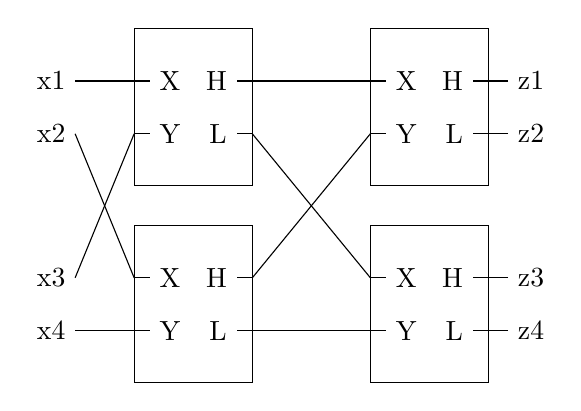
\begin{tikzpicture}
    \compareBlock[name=inL]{(0, 0)}
    \compareBlock[name=inU]{(0, 2.5)}
    \compareBlock[name=outL]{(3, 0)}
    \compareBlock[name=outU]{(3, 2.5)}
    \connectCB{inU_l}{outL_a}{black}
    \connectCB{inL_l}{outL_b}{black}
    \connectCB{inU_h}{outU_a}{black}
    \connectCB{inL_h}{outU_b}{black}

    \inputCB{inU}{x1}{x2}
    \inputCB{inL}{x3}{x4}
    \outputCB{outU}{z1}{z2}
    \outputCB{outL}{z3}{z4}

    \connectCB{x1}{inU_a}{black}
    \connectCB{x2}{inL_a}{black}
    \connectCB{x3}{inU_b}{black}
    \connectCB{x4}{inL_b}{black}
\end{tikzpicture}


\begin{tikzpicture}
    \compareBlock[name=inL, a=2, b=4, ca=blue, cb=pink]{(0, 0)}
    \compareBlock[name=inU, a=1, b=3, ca=red, cb=green]{(0, 2.5)}
    \compareBlock[name=outL]{(3, 0)}
    \compareBlock[name=outU]{(3, 2.5)}
    \connectCB{inU_l}{outL_a}{black}
    \connectCB{inL_l}{outL_b}{black}
    \connectCB{inU_h}{outU_a}{black}
    \connectCB{inL_h}{outU_b}{black}

    \inputCB{inU}{1}{2}
    \inputCB{inL}{3}{4}
    \outputCB{outU}{z1}{z2}
    \outputCB{outL}{z3}{z4}

    \connectCB{x1}{inU_a}{red}
    \connectCB{x2}{inL_a}{blue}
    \connectCB{x3}{inU_b}{green}
    \connectCB{x4}{inL_b}{pink}
\end{tikzpicture}

\begin{tikzpicture}
    \compareBlock[name=inL, a=2, b=4, h=4, l=2, ca=blue, cb=pink, cl=blue, ch=pink]{(0, 0)}
    \compareBlock[name=inU, a=1, b=3, h=3, l=1, ca=red, cb=green, cl=red, ch=green]{(0, 2.5)}
    \compareBlock[name=outL, a=1, b=2, ca=red, cb=blue]{(3, 0)}
    \compareBlock[name=outU, a=3, b=4, ca=green, cb=pink]{(3, 2.5)}
    \connectCB{inU_l}{outL_a}{red}
    \connectCB{inL_l}{outL_b}{blue}
    \connectCB{inU_h}{outU_a}{green}
    \connectCB{inL_h}{outU_b}{pink}

    \inputCB{inU}{1}{2}
    \inputCB{inL}{3}{4}
    \outputCB{outU}{z1}{z2}
    \outputCB{outL}{z3}{z4}

    \connectCB{x1}{inU_a}{red}
    \connectCB{x2}{inL_a}{blue}
    \connectCB{x3}{inU_b}{green}
    \connectCB{x4}{inL_b}{pink}
\end{tikzpicture}

\begin{tikzpicture}
    \compareBlock[name=inL, a=2, b=4, h=4, l=2, ca=blue, cb=pink, cl=blue, ch=pink]{(0, 0)}
    \compareBlock[name=inU, a=1, b=3, h=3, l=1, ca=red, cb=green, cl=red, ch=green]{(0, 2.5)}
    \compareBlock[name=outL, a=1, b=2, ca=red, cb=blue  , h=2,l=1,ch=blue,cl=red]{(3, 0)}
    \compareBlock[name=outU, a=3, b=4, ca=green, cb=pink, h=4,l=3,ch=pink,cl=green]{(3, 2.5)}
    \connectCB{inU_l}{outL_a}{red}
    \connectCB{inL_l}{outL_b}{blue}
    \connectCB{inU_h}{outU_a}{green}
    \connectCB{inL_h}{outU_b}{pink}

    \inputCB{inU}{1}{2}
    \inputCB{inL}{3}{4}
    \outputCB{outU}{z1}{z2}
    \outputCB{outL}{z3}{z4}

    \connectCB{x1}{inU_a}{red}
    \connectCB{x2}{inL_a}{blue}
    \connectCB{x3}{inU_b}{green}
    \connectCB{x4}{inL_b}{pink}
\end{tikzpicture}

\section{Bitonic Sorter}

With a bitonic sorter only bitonic sequences can be used as inputs.
In order to sort arbitrary input sequences a bitonic sorting network can be created from bitonic sorters.
For bitonic sorting networks see the next chapter.

A bitonic sorter for k=1 (n=2) is trivially just a comparator. 
Which we illustrate by using the given box layout with X and Y being the inputs and H the higher output and L the lower output respectivly.

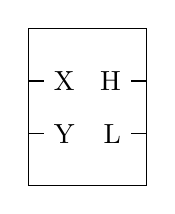
\begin{tikzpicture}
    \compareBlock[name=inL]{(0, 0)}
\end{tikzpicture}

With the sorter for k=1 we can recursivly create a sorter of higher order.
For example consider the following k=2 (n=4) bitonic sorter.

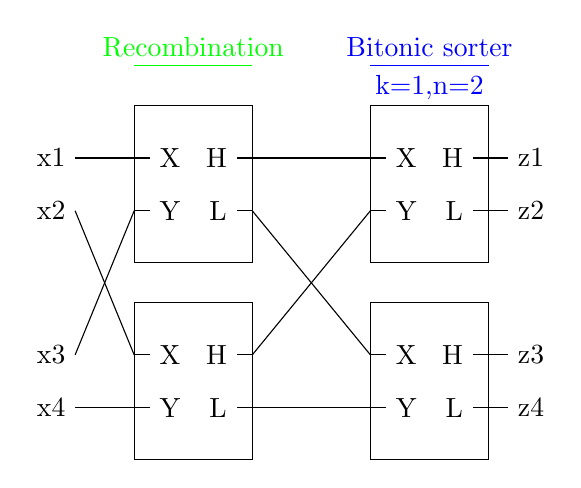
\begin{tikzpicture}
    \draw[color=blue] (3, 5) -- node[above] {Bitonic sorter} node[below] {k=1,n=2} (4.5, 5);
    \draw[color=green] (0, 5) -- node[above] {Recombination} (1.5, 5);

    \compareBlock[name=inL]{(0, 0)}
    \compareBlock[name=inU]{(0, 2.5)}
    \compareBlock[name=outL]{(3, 0)}
    \compareBlock[name=outU]{(3, 2.5)}
    \connectCB{inU_l}{outL_a}{black}
    \connectCB{inL_l}{outL_b}{black}
    \connectCB{inU_h}{outU_a}{black}
    \connectCB{inL_h}{outU_b}{black}

    \inputCB{inU}{x1}{x2}
    \inputCB{inL}{x3}{x4}
    \outputCB{outU}{z1}{z2}
    \outputCB{outL}{z3}{z4}

    \connectCB{x1}{inU_a}{black}
    \connectCB{x2}{inL_a}{black}
    \connectCB{x3}{inU_b}{black}
    \connectCB{x4}{inL_b}{black}
\end{tikzpicture}

The bitonic sorter consist of two layers a recombination layer and bitonic sorters of a lower order.
The recombination layer recombines the bitonic inputs into two new bitonic sequences who are half as big as the original sequence.
In the bitonic sort layer there are two bitonic sorters of order k-1 how take the again bitonic input of the recombination and sort them.

This can be done recursivly for each k using an input of each monotonic sequence per comparator.
The following illustration shows the connection of the recombination in order for this two work.



\section{Sorting network}

A bitonic sorting network is created by using several bitonic sorter. 
These bitonic sorters are recursivly used to create two monotonic one decreasing and one increasing sequence who are then put into the next stage.
This creates a bitonic series for the next stage which can then use this bitonic series to be used as a monotonic series for the next stage.
Consider the following example for a n=4 bitonic sort network.

\begin{tikzpicture}
    
    \draw[color=black] (-2.25, 6) -- node[above] {Bitonic sorting network} node[below] {k=2,n=4} (4.5, 6);
    \draw[color=blue] (0, 5) -- node[above] {Bitonic sorter} node[below] {k=2,n=4} (4.5, 5);
    \draw[color=green] (-2.25, 5) -- node[above] {Sorter} node[below] {k=1} (-0.75, 5);

    \draw[->,color=orange] (-2.5, 4.5) -- node[left] {increasing} (-2.5, 2.5);
    \draw[<-,color=orange] (-2.5, 2) -- node[left] {decreasing} (-2.5, 0);

    \compareBlock[name=inL]{(0, 0)}
    \compareBlock[name=inU]{(0, 2.5)}
    \compareBlock[name=outL]{(3, 0)}
    \compareBlock[name=outU]{(3, 2.5)}
    \compareBlock[name=preL, l=H, h=L]{(-2.25, 0)}
    \compareBlock[name=preU]{(-2.25, 2.5)}

    \connectCB{inU_l}{outL_a}{black}
    \connectCB{inL_l}{outL_b}{black}
    \connectCB{inU_h}{outU_a}{black}
    \connectCB{inL_h}{outU_b}{black}

    \outputCB{outU}{z1}{z2}
    \outputCB{outL}{z3}{z4}

    \connectCB{x1}{inU_a}{black}
    \connectCB{x2}{inL_a}{black}
    \connectCB{x3}{inU_b}{black}
    \connectCB{x4}{inL_b}{black}
\end{tikzpicture}

The bitonic sorting network for k=2 can be created by using a k=2 bitonic sorter and two k=k-1 sorter.
The two sorter create a decreasingly or increasingly sorted sequence in order to create a bitonic input for the bitonic sorter.
Bitonic sorting networks of a lower order are mostly used for the two pre sorters, therefore a recursiv definition of a bitonic sorting network from bitonic sorters can be descibed.
In the above example the two bitonic sorting networks are k=1 networks hence they are just a comparator.



\end{document}